\documentclass[a4paper,12pt]{article}
\usepackage{setspace}
\usepackage{cmap}					
\usepackage{mathtext} 				
\usepackage[T2A]{fontenc}			
\usepackage[utf8]{inputenc}			
\usepackage[english,russian]{babel}
\usepackage{multirow}
\usepackage{graphicx}
\usepackage{wrapfig}
\usepackage{tabularx}
\usepackage{float}
\usepackage{longtable}
\usepackage{graphicx}
\usepackage{hyperref}
\hypersetup{colorlinks=true,urlcolor=blue}
\usepackage[rgb]{xcolor}
\usepackage{amsmath,amsfonts,amssymb,amsthm,mathtools} 
\usepackage{icomma} 
\mathtoolsset{showonlyrefs=true}
\usepackage{euscript}
\usepackage{mathrsfs}

\title{Статистики Ферми-Дирака и Бозе-Эйнштейна}
\author{Мадорский Кирилл}
\date{10 июня 2023}
\maketitle

\begin{document}


\subsection*{Введение}
\par\indent\indentВ рамках статистической физики важную роль в описании термодинамических систем играет поиск наиболее достоверной модели распределения частиц по скоростям и энергиям. С помощью понятий микро- и макросостояний системы, данная задача сводится к определению такого распределения, при котором её статистический вес примет максимальное значение, что эквивалентно наиболее вероятному (или равновесному) состоянию. При этой формулировке становится очевидно, что искомое распределение зависит от того, как мы определим статистический вес системы. Неочевидность данного выбора породила три основных модели распределений, о которых далее пойдет речь - статистики Больцмана, Ферми-Дирака и Бозе-Эйнштейна.


\subsection*{Бозоны и фермионы}
\par\indent\indentВажно упомянуть тот факт, что статистики Ферми-Дирака и Бозе-Эйнштейна, хоть и подлежат сравнению, однако не являются взаимо-исключающими моделями, так как применяются для описания различных термодинамических систем. Согласно квантовой теории, все частицы разделяюстя на два класса. К первому относятся электроны, протоны, нейтроны и все частицы с полуцелым спином -- фермионы. Ко второму классу относятся бозоны -- частицы с целым спином, такие как фотоны, глюоны и K-мезоны. Для описания фермионов используется статистика Ферми-Дирака, а для бозонов -- Бозе-Эйнштейна. Как будет видно далее, статистика Больцмана является их приближенным предельным вариантом.
\newpage

\subsection*{Тождественность}
\par\indent\indentВо всех трех статистиках микросостояния системы принимаются равновероятными, однако определяется микросостояние по-разному. В основе статистики Больцмана лежит принцип различимости частиц, будь они даже абсолютно тождественны. В связи с этом при перестановке двух частиц получается новое микросостояние. В статистиках же Ферми-Дирака и Бозе-Эйнштейна заложен противоположный принцип абсолютной неразличимости частиц, что приводит к меньшему числу возможных микросостояний. В чём же различие между статистиками Ферми-Дирака и Бозе-Эйнштейна? В первом случае принимается, что в каждом квантовом состоянии может находиться лишь одна частица, в то время как вторая статистика таких ограничений не накладывает. Проиллюстрируем эти различия рисунком. Пусть две частицы необходимо разделить по трём квантовым состояниям. Будем изображать состояния клетками, а частицы - буквами или точками.

\begin{figure}[h!]
\centering
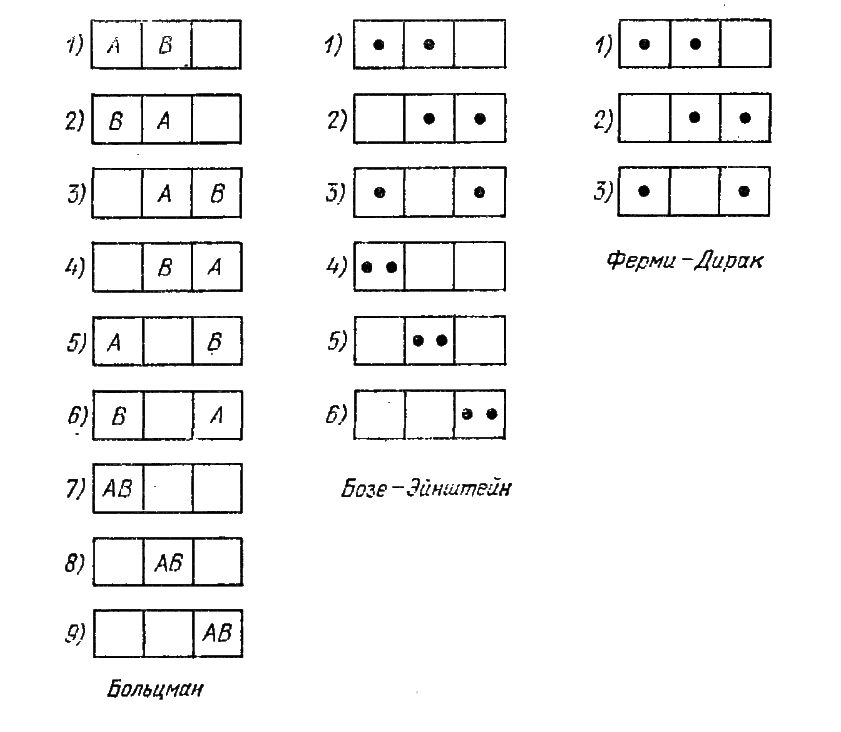
\includegraphics[width=0.9\textwidth]{cells.png}
\caption{Распределение 2 частиц по 3 состояниям }
\end{figure}
\newpage

Цифрами пронумерованы микросостояния. Как видно, по статистике Больцмана микросостояния 1 и 2 различны, тогда как для статистики Бозе-Эйнштейна и Ферми-Дирака это состояние под номером 1. Для фермионов 4, 5 и 6 состояния недоступны, остаются только микросостояния, обозначенные в правом столбце. В силу равнодоступности микросостояний изменяются и математические вероятности каждого: одно и то же состояние в статистике Ферми-Дирака имеет вероятность 1/3, в статистике Бозе-Эйнштейна 1/6 и в статистике Больцмана 2/9.



\subsection*{Комбинаторика распределения}
\par\indent\indentРешим две комбинаторные задачи -- сколькими способами $N$ тождественных частиц можно разместить по $Z$ квантовым состояниям?
\begin{wrapfigure}{r}{0.35\textwidth}
  \begin{center}
    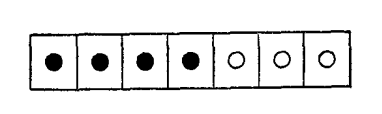
\includegraphics[width=0.4\textwidth]{ferm.png}
  \end{center}
\end{wrapfigure}
\par\indent\indentПусть частицы -- фермионы. Тогда $N\leq Z$, иначе распределение невозможно в силу ограничения на число частиц "в одной ячейке". Изобразим квантовые состояния клетками, заполненные клетки отметим черными кружками, остальные белыми. Всевозможных перестановок клеток $Z!$, однако в силу тождественности перестановки черных и белых кружков не меняют распределения, их соответственно $N!$ и $(Z-N)!$. Получаем итоговое количество способов расстановки фермионов
\[\frac{Z!}{N!(Z-N)!}\]
\begin{wrapfigure}{H!}{0.35\textwidth}
  \begin{center}
    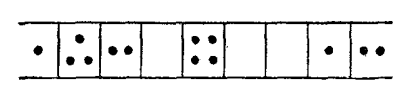
\includegraphics[width=0.35\textwidth]{boz.png}
  \end{center}
\end{wrapfigure}
\par\indent\indentАналогичным образом задача решается для бозонов.
Чтобы разбить $N$ частиц на $Z$ групп необходимо расставить $Z-1$ перегородок, то есть на этот раз элементов в ряду $Z+N-1$. Однако как и в предыдущем случае перегородки и частицы неразличимы, то есть полное число перестановок надо поделить на число перестановок перегородок и частиц. В итоге получаем формулу
\[\frac{(Z+N-1)!}{N!(Z-1)!}\]




\newpage
\subsection*{Распределения Ферми-Дирака и Бозе-Эйнштейна}
\par\indent\indentРешив эти задачи можно перейти к выводу распрелений. Обозначим условия: рассматриваем идеальный газ фермионов или бозонов, помещенный в сосуд постоянного объема с твердыми, адиабатическими стенками. Чтобы охарактеризовать макросостояние газа, разделим все квантовые состояния частицы на узкие энергетические слои. Каждый такой слой будет соответствовать множеству квантовых состояний с одинаковыми или очень близкими энергиями частицы в диапазоне $(\varepsilon_i, \varepsilon_i+ \delta{\varepsilon_i})$, где $\delta{\varepsilon_i} \ll \varepsilon_i$. Кроме того, число квантовых состояний $Z_i$ в одном слое должно быть велико. Тогда макросостояние газа характеризуется заданием чисел $N_i$ частиц в одном слое. Воспользовавшись решением задач из предыдущего параграфа получаем число способов размещения $N_i$ частиц по $Z_i$ квантовым состояниям i-го слоя:
\[G_i = \frac{Z_i!}{N_i!(Z_i-N_i)!} \hspace{10px}\text{ или }\hspace{10px} G_i = \frac{(Z_i+N_i-1)!}{N_i!(Z_i-1)!}\]
для фермионов и бозонов соответственно. В силу независимости слоев, перемножая все $G_i$ найдем статистический вес данного макросостояния газа
\[G = \prod_i\frac{Z_i!}{N_i!(Z_i-N_i)!} \hspace{10px}\text{ и }\hspace{10px} G = \prod_i\frac{(Z_i+N_i-1)!}{N_i!(Z_i-1)!}\]

\par\indent\indentОпределив статистические веса можем решить задачу об их максимизации, то есть нахождении распределения в равновесном положении. Полагая все $Z_i$ и $N_i$ большими значениями, воспользуемся приближенной формулой Стирлинга при вычислении энтропии:
\begin{equation*}
 \begin{cases}
   lnN! = NlnN - N\\
   S = kln{G}
 \end{cases}
\end{equation*}
\begin{equation*}
 \begin{cases}
   S_\text{ф} = -k\sum{[N_ilnN_i + (Z_i-N_i)ln(Z_i-N_i)]+const}\\
   S_\text{б} = k\sum{[(Z_i+N_i-1)ln(Z_i+N_i-1) - N_ilnN_i]+const}
 \end{cases}
\end{equation*}
Используем условия сохранения полной энергии и полного числа частиц для поиска минимума энтропии:
\begin{equation*}
 \begin{cases}
    \sum{dN_i} = 0\\
    \sum{\varepsilon_i dN_i} = 0\\
    \sum{ln\frac{N_i}{Z_i - N_i}dN_i} = 0 & \text{для фермионов}\\
    \sum{ln\frac{N_i}{Z_i + N_i-1}dN_i} = 0 & \text{для бозонов}\\
 \end{cases}
\end{equation*}
\newpage
\par\indent\indentИз этих соотношений получаем зависимость $N_i$ от $\varepsilon_i$:
\[\frac{N_i}{Z_i-N_i} = Ae^{-\alpha\varepsilon_i} \hspace{10px}\text{ и }\hspace{10px} \frac{N_i}{Z_i+N_i} = Ae^{-\alpha\varepsilon_i}\]
Здесь коэффициент $\alpha$ имеет то же значение, что и в распределении Больцмана, и получается аналогичным выводом (за счёт перераспределения частиц по слоям меняется енергия системы, связанная с изменением энтропии через температуру и постоянную Больцмана).
\[\alpha = \frac{1}{kT}\]
\par\indent\indentПолученные формулы можно переписать в ином виде, выразив среднее число частиц $\overline{n_i}$, приходящееся на одно квантовое состояние.
\[\overline{n_i} = \frac{1}{\text{exp}\frac{\varepsilon_i-\mu}{kT}+1} \hspace{10px}\text{для фермионов}\]
\[\overline{n_i} = \frac{1}{\text{exp}\frac{\varepsilon_i-\mu}{kT}-1} \hspace{10px}\text{для бозонов}\]

Данные распределения и называются распределениями Ферми-Дирака и Бозе-Эйнштейна. Параметр $\mu$ связан с $A$ соотношением $\mu = kTlnA$.

\subsection*{Связь с распределением Больцмана}
\par\indent\indentИз формул распределений следует, что при малых числах заполнений, то есть при $\overline{n_i} \ll 1$ формулы переходят в формулу распределения Больцмана: 
\[\overline{n_i} = \text{exp}\frac{\mu-\varepsilon_i}{kT} = \text{const}\cdot\text{exp}\frac{-\varepsilon_i}{kT}\]

\subsection*{Химическйи потенциал}
\par\indent\indentНа примере ферми-газа покажем, что константа $\mu$ имеет смысл химического потенциала. Воспользуемся выражением для энтропии ферми-газа, полученным ранее. При этом будем менять число частиц газа, оставляя неизменными его температуру и объем.
\[dS = -k\sum_i{ln\frac{N_i}{Z_i-N_i}dN_i}\]
В состоянии равновесия согласно статистике Ферми-Дирака
\[ln\frac{N_i}{Z_i-N_i} = \frac{\mu-\varepsilon_i}{kT}\]
Таким образом,
\[dS = -k\sum_i\frac{\mu-\varepsilon_i}{kT}dN_i = -\frac{\mu}{T}\sum_idN_i + \sum_i\frac{\varepsilon_i}{T}dN_i\]
\[TdS = dU - \mu dN\]
\[\mu = (\frac{d\Psi}{dN})_{T,V}\]
Из последнего равенства видно, что $\mu$ -- химический потенциал газа.


\subsection*{Графики распределений}
\par\indent\indentРаспределение Ферми-Дирака зависит температуры, объема и числа частиц, но при замкнутости системы имеет вид, изображенный на графике:
\begin{figure}[h!]
\centering
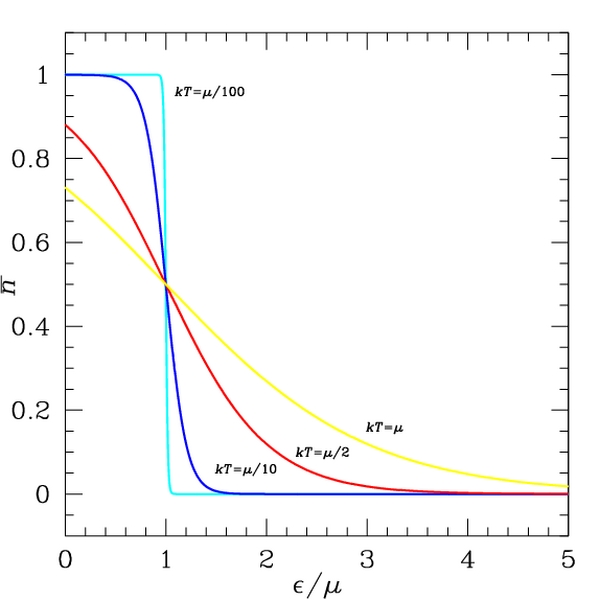
\includegraphics[width=0.8\textwidth]{fgr.jpg}
\caption{Распределение Ферми-Дирака}
\end{figure}
\newpage

\par\indent\indentИнтересно, что при $T\rightarrow 0$ распределение выраждается, и частицы ферми-газа заполняют все квантовые состояния с энергиями $\varepsilon_i < \mu$. Сравнение распределений Больцмана, Ферми-Дирака и Бозе-Эйнштейна приведено на следующем рисунке. 
\begin{figure}[h!]
\centering
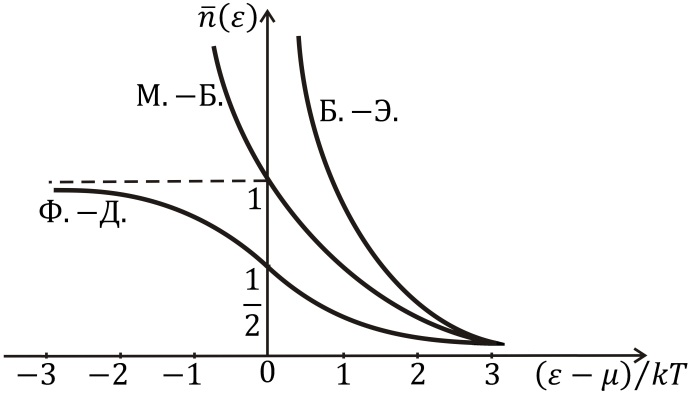
\includegraphics[width=1\textwidth]{bfe1.jpg}
\caption{Сравнение распределений}
\end{figure}


\subsection*{Заключение}
\par\indent\indentДля применения распределений Ферми-Дирака и Бозе-Эйнштейна надо знать выражения для энергий и соответствующих им чисел квантовых состояний, что делает их неудобными в решении некоторых задач, однако области применения статистик весьма обширны. Статистика Ферми-Дирака используется для описания электронных свойств металлов и полупроводников, таких как транзисторы и диоды. Она также используется в теории ядерных реакций и при описании поведения кварков. Статистика Бозе-Эйнштейна используется в физике конденсированного состояния для описания свойств квантовых газов, в теории сверхпроводимости и при изучении свойств лазеров и магнитных резонансов. Кроме того, статистики Ферми-Дирака и Бозе-Эйнштейна применяются в различных областях, таких как космология, астрофизика, биофизика и экономика.
\end{document}